%!TEX encoding = UTF-8 Unicode
%!TEX TS-program = xelatex

\documentclass[a4paper,11pt]{article}
\usepackage{CLARIN2024}
% - - - - - - - IMPORTANT - - - - - - - -
% The next three lines allow XeLaTeX, graphics import and hyperlinks, set font and language
%\usepackage{xltxtra,polyglossia,graphicx,hyperref}
%\setmainfont[Mapping=tex-text]{Times}
%\setdefaultlanguage{english}
% If for some reason the above three lines are not compatible with your LaTeX installation,
% comment out the above three instructions and uncomment the following four instead:
\usepackage{times}
\usepackage{url}
\usepackage{latexsym}
\usepackage{hyperref}
\usepackage{graphicx}
\usepackage[english]{babel}
\usepackage{csquotes}
\usepackage[
    backend=biber,
    style=apa,
    natbib=true,
    ]{biblatex}
\addbibresource{tooldiscovery.bib} % add your own bibliography into the format provided in this file

%\setlength\titlebox{5cm}

% You can expand the titlebox if you need extra space
% to show all the authors. Please do not make the titlebox
% smaller than 5cm (the original size); we will check this
% in the camera-ready version and ask you to change it back.

%\usepackage{covington} % if needed, for linguistic examples

\title{FAIR Tool Discovery: an automated software metadata harvesting pipeline for CLARIAH}

% - - - - - - - IMPORTANT - - - - - - -
% Leave the author information empty until your paper has been accepted 

% Uncomment the following line ONLY if you need two author rows
%\setlength\titlebox{80mm} 

\author{Maarten van Gompel \\
  KNAW Humanities Cluster \\
  Amsterdam, the Netherlands \\
  {\tt proycon@anaproy.nl} \\\And % if needed: this makes a second column
  Second Author \\
  Department (optional)\\
  University Name without city \\
  City, Country \\
 {\tt email@domain} \\
% \AND % if needed: this makes a second row
%  Third Author \\
%  Department (optional)\\
%  University of City, Country \\
%  {\tt email@domain} \\\And
%  Fourth Author \\
%  Department (optional)\\
%  University Name without city \\
%  City, Country \\
%  {\tt email@domain} \\
} 

\date{}

\begin{document}
\maketitle
\begin{abstract}
  We present the Tool Discovery pipeline, a core component of the CLARIAH
    infrastructure in the Netherlands. This pipeline harvests software metadata
    from the source, detects existing heterogeneous metadata formats already in
    use by software developers, and converts it to a uniform representation
    based on schema.org and codemeta. The resulting data is then made available
    for further ingestion into other user-facing catalogue/portal systems. 
\end{abstract}

\section{Introduction} \label{intro}

% - - - - - - - IMPORTANT - - - - - - -
% The following footnote without marker is needed for the camera-ready
% version of the paper.
% Comment out the instructions (first text) and uncomment the 8 lines
% under "final paper" for your variant of English.
%
\blfootnote{
    %
    % for review submission
    %
    %\hspace{-0.65cm}  % space normally used by the marker
This work is licenced under a Creative Commons Attribution 4.0 International Licence. Licence details: {http://creativecommons.org/licenses/by/4.0/}
    % % final paper: en-uk version (to license, a licence)
    %
    % \hspace{-0.65cm}  % space normally used by the marker
    % This work is licensed under a Creative Commons
    % Attribution 4.0 International Licence.
    % Licence details:
    % {http://creativecommons.org/licenses/by/4.0/}
    %
    % % final paper: en-us version (to licence, a license)
    %
    % \hspace{-0.65cm}  % space normally used by the marker
    % This work is licenced under a Creative Commons
    % Attribution 4.0 International License.
    % License details:
    % {http://creativecommons.org/licenses/by/4.0/}
}

% Software is indispensible in a lot of modern-day research, including in sectors
% such as the Humanities and Social Sciences that may have traditionally been
% less focused on information technology. It is also appreciated more and more as
% valid research output, alongside more conventional output such as academic
% publications, presentations, and datasets. Scholars often have a need for
% research software to do their research efficiently.

For scholars it is important to be able to find and identify tools
suitable for their research, we call this \emph{tool discovery}. We define
\emph{tool} here and throughout this paper to broadly refer to any kind of
software, regardless of the interface it offers and the audience it targets.
The scholar's requirement to find tools is reflected in the letter \textsc{F}
for \emph{Findable} in the ubiquitous acronym \textsc{FAIR} \footnote{Findable,
Accessible, Interoperable and Reusable} that has received a lot of attention in
recent years in academic circles and is also adopted to promote quality and
sustainability in research software \citep{FAIR}. In order to find tools,
researchers must have access to catalogues that relay \emph{accurate} software
metadata.

There is no shortage in existing initiatives in building such catalogues\footnote{CLARIN itself has one in the form of the Virtual Language Observatory: \url{https://vlo.clarin.eu} \citep{VLO}}.
, %<cut out part below for brevity>
but the system we describe in this paper is not an attempt to build another catalogue.
We developed a generic pipeline that harvests software metadata from the source, leveraging
various existing metadata formats, and converts it to a uniform linked open data representation.
This we then make available for further ingestion into catalogues. 

%; many
%research groups, projects or institutes have some kind of website featuring
%their tools. Aggregation of software metadata from multiple such partners is
%also not new, as CLARIN itself already does in the CLARIN Virtual Language
%Observatory\footnote{\url{https://vlo.clarin.eu}} \citep{VLO}.


\section{The need for high-quality metadata}

Unlike most digital data, software is uniquely characterised as a constantly
moving target. Releases address bugs, security vulnerabilities, or add new
features. Moreover, software lives not in isolation, but in connection to other
software; its dependencies. Updates are needed to adapt to changes in its
environment.

For software metadata to be informative in this dynamic setting, it needs to
explicitly link to a particular version of the software. This is also
facilitates provenance keeping and scientific reproducibility. Metadata should
also convey information about the stage of development the software is in and
the level of support an end-user may expect. The user would be wise to exercise
caution in adopting software that is unmaintained and unsupported. In practice
we often find this information lacking and come across catalogues that were
manually compiled once but rarely updated since.

The need for accurate up-to-date metadata goes hand-in-hand with the need for
\emph{complete} metadata. If vital details are missing, the
end-user may not be able to make an informed judgment.

% A common pitfall we have observed in practice is that metadata is often
% manually collected at some stage and published in a catalogue, but never or
% rarely updated or revised. In best case, the software has moved on and the
% metadata covers a mere subset, in worst case, the software or the entire
% catalogue is unmaintained and out of date.

\section{Bottom-up harvesting from the source}

What we propose is a \emph{fully automated} pipeline where software metadata is
kept at the source, i.e. alongside the software source code, and \emph{periodically} harvested from there\footnote{Formally, the software source code has
no knowledge when, where, and by whom it may be deployed as a service. This linking is
therefore established at a higher level.}. This has a number of important advantages: 
%and can be contrasted with metadata that lives primarily in an intermediate system.

%\begin{itemize}

%\item

Source code is often already accompanied by software metadata in existing
schemas\footnote{for example \texttt{pyproject.toml}, \texttt{setup.py}, \texttt{pom.xml}, \texttt{package.json}, \texttt{CITATION.cff} and others. Even files such as \texttt{README} and \texttt{LICENSE} may be a source for certain metadata.} because many programming language ecosystems already either require or
recommend this. Our aim is to avoid any duplication of metadata and
\emph{reuse} these existing sources to the maximum extent possible.

%Consider
%for example \texttt{pyproject.toml} or \texttt{setup.py} for Python projects,
%\texttt{package.json} for javascript/npm/nodejs projects, \texttt{pom.xml} for
%Java/Maven and \texttt{Cargo.toml} for Rust. Aside from these, valuable machine
%parsable metadata may be extracted from other files such as a \texttt{LICENSE}
%file or , `README` file which often contains machine-interpretable
%badges\footnote{Badges are small images often included on top a \texttt{README}
%file to express certain properties of the software, such as links to
%documentation, continuous integration services, development status, packaging
%status, etc..}, or a \texttt{CITATION.cff} file, amongst others. Multiple such
%sources may be present and can be recombined.

%\item 
  Second, source code should be under version control (e.g. git) and published in a forge (e.g. GitHub).
  %  is typically held in a version control system (usually git) and published in 
  %forges such as Github, Gitlab, Bitbucket, Codeberg or Sourcehut.
  This solves versioning issues and ensures metadata can exactly describe the version alongside which it is stored. It also enables the 
  harvester to properly identify the latest stable release\footnote{provided some kind of industry-standard versioning system like semantic versioning is adhered to}.
  Software forges themselves may also provide an API that may serve as an extra source to find software metadata (e.g. descriptions, keywords, links to issue trackers and/or continuous integration services).
%\item 
  Third, The developers of the tool have full control and authorship over their metadata. There are no middlemen.
%\item 
  Last, the forges were designed precisely for collaboration on open source software development, so mechanisms for any
  third party to amend or correct the metadata are already in place (e.g. via a pull/merge request or patches).
  So while developers retain full authorship, this does not mean curation is not possible.
%\end{itemize}

We do not harvest any metadata from intermediaries\footnote{other catalogues, for instance via PMI-OAI
endpoints} as that would defeat our philosophy. We do have one extra source for
harvesting: In case the tool in question is Software as a Service, i.e. a
web-application, web-service, or website, we harvest not only the software
source code, but also a web endpoint and attempt to automatically extract
metadata from there. In the resulting metadata, there will be an explicit link
between the source code and any \emph{target products} or \emph{instances} of
that source code. The sources for harvesting source repositories and web
endpoints (URLs) are the only input that needs to be manually provided to our
system, we call this the \emph{source registry} and we keep this in a simple
git repository containing very minimalistic configuration files (one per tool).
This is also the only point in our pipeline where there is the possibility for
human supervision; to decide whether or not to include a tool.

\section{A unified vocabulary for software metadata}

The challenge we are facing is primarily one of mapping from multiple
heterogeneous sources of software metadata to a unified vocabulary.
Fortunately, this is an area that has been explored previously in the CodeMeta
project\footnote{\url{https://codemeta.github.io}}. They developed a
vocabulary for describing software source code, building on top of the
schema.org vocabulary and contributing their efforts back to them. Moreover,
the CodeMeta project defines mappings, called crosswalks, between their
vocabulary and many existing metadata schemes. 

Schema.org and codemeta are both linked open data (LOD) vocabularies\footnote{i.e.
building upon RDF and being retrievable over HTTP}, and codemeta is canonically
serialised to a JSON-LD file which makes it easily parsable for both machine
and human alike. This \texttt{codemeta.json} file can be kept under version
control alongside a tool's source code. 

We link to various other LOD vocabularies, such as
\emph{repostatus.org}\footnote{\url{https://repostatus.org}} (development
status), \emph{SPDX}\footnote{\url{https://spdx.dev}} (open source software
licenses), \emph{TaDiRaH}\footnote{\url{https://vocabs.dariah.eu/tadirah/}}
(research activities) \citep{TADIRAH} and \emph{NWO Research Domains}.
Moreover, we formulated some of our own extensions on top of codemeta and
schema.org, such as Software
Types\footnote{\url{https://github.com/SoftwareUnderstanding/software_types}},
Software Input/Output
Data\footnote{\url{https://github.com/SoftwareUnderstanding/software-iodata}},
and Research Technology Readiness Levels. Most of these are formulated as SKOS
vocabularies.

\section{Architecture}

The full architecture of our pipeline is illustrated schematically in
Figure~\ref{fig:architecture}. While we demonstrate this in the context of the
CLARIAH project, the underlying technology is generic and can be reapplied in
other projects as well.

\begin{figure}[h]
\begin{center}
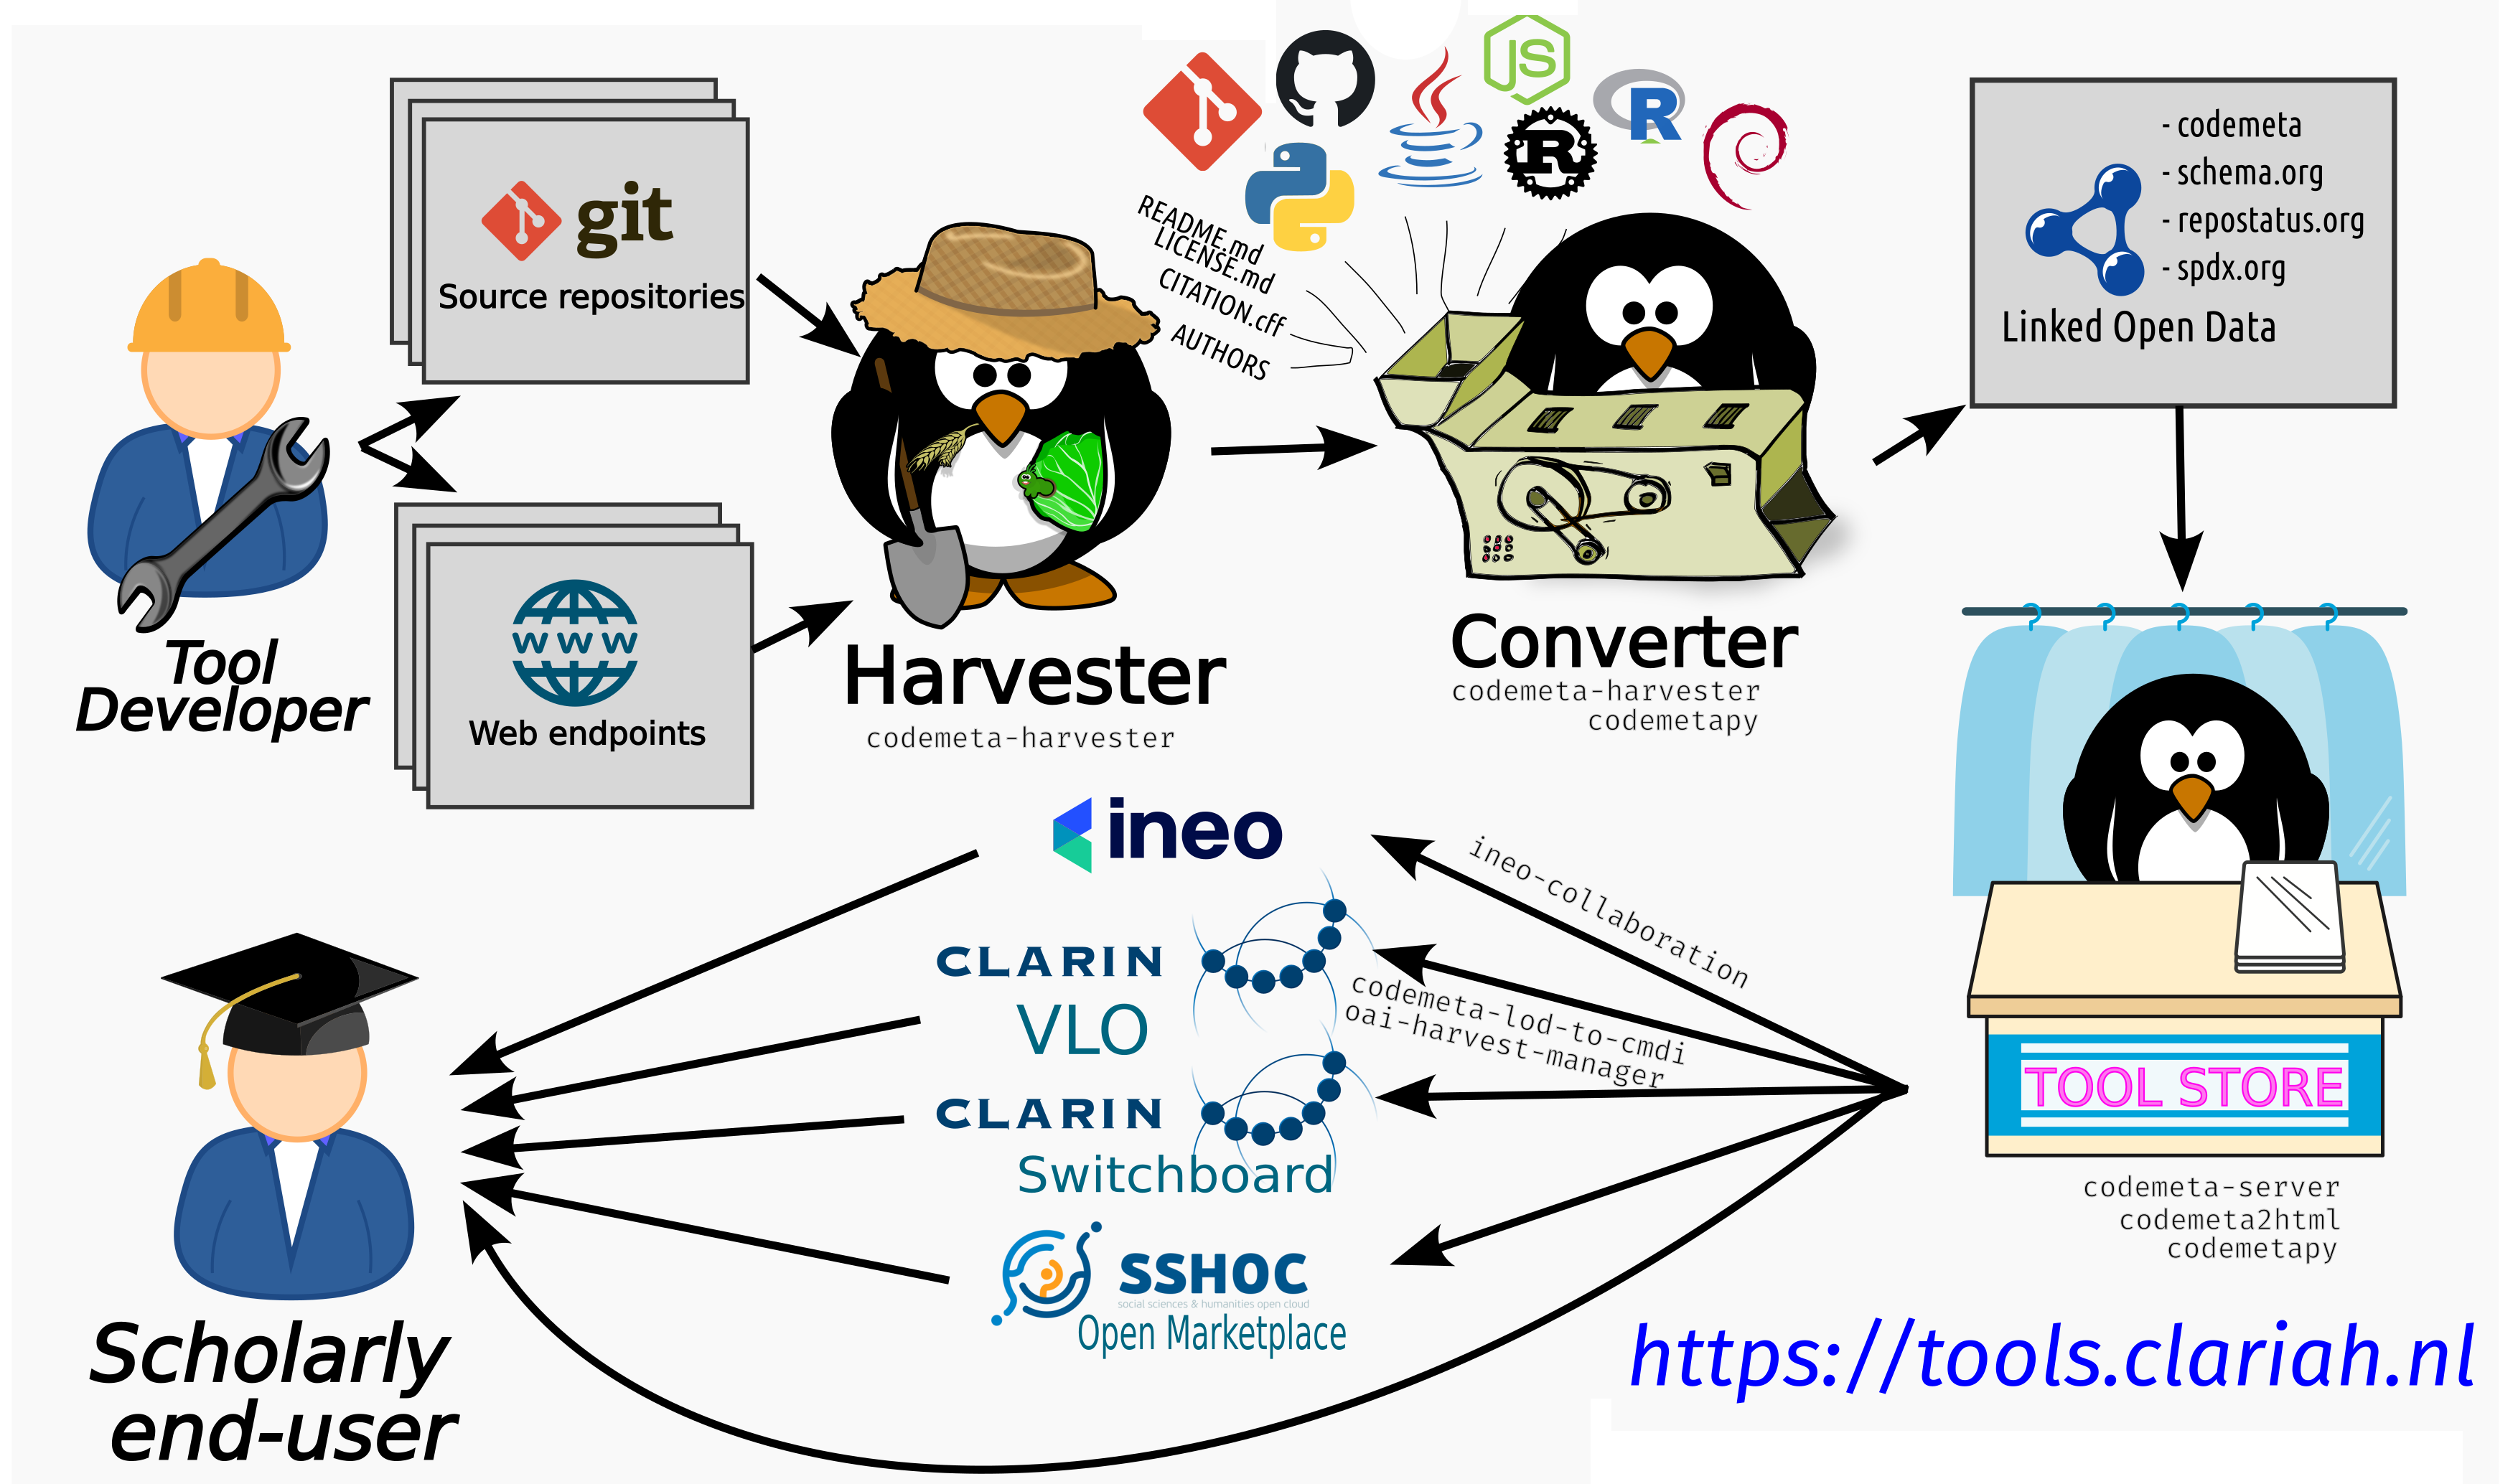
\includegraphics[width=14.0cm]{architecture.png}
\caption{The CLARIAH Tool Discovery architecture}
\end{center}
\label{fig:architecture}
\end{figure}

Using the input from the source registry, our
\emph{harvester}\footnote{codemeta-harvester:
\url{https://github.com/proycon/codemeta-harvester}} fetches all the git
repositories and queries any service endpoints. It does so at regular intervals
(e.g. once a day). This ensures the metadata is always up to date. When the
sources are retrieved, it identifies the different kinds of metadata it can
find there and and calls the converter\footnote{powered by codemetapy:
\url{https://github.com/proycon/codemetapy}} to turn and combine it into a
single codemeta representation. This produces one codemeta JSON-LD file per
input tool. All of these together are loaded in our \emph{tool store}. This is
implemented as a triple store and servers both as a backend to be queried
programatically using SPARQL, as well as a simple web frontend to be visited by
human end-users as a catalogue \footnote{codemeta-server
(\url{https://github.com/proycon/codemeta-server}) and codemeta2html
(\url{https://github.com/proycon/codemeta2html}). The results for CLARIAH are
accessible at \url{https://tools.clariah.nl}}.

Our web frontend is not the final destination; our aim is to propagate the
metadata we have collected to other existing portal/catalogue systems, such as
the CLARIN VLO, the CLARIN
Switchboard\footnote{\url{https://switchboard.clarin.eu/}}, the SSHOC
Marketplace\footnote{\url{https://marketplace.sshopencloud.eu/}}, and CLARIAH's
Ineo\footnote{\url{https://ineo.tools}}.

\section{Validation \& Curation}

Having an automated metadata harvesting pipeline may raise some concerns
regarding quality assurance. Data is automatically converted from heterogeneous
sources and immediately propagated to our tool store, this is not withotu
error. In absence of human curation, which is explicitly out of our intended
scope, we tackle this issue through an automatic validation mechanism.

The harvested codemeta metadata is held against a validation
schema\footnote{formulated in SHACL} that tests whether certain fields are
present (completeness), and whether the values are sensible (accuracy, it is
capable of detecting various discrepancies). The validation process outputs a
human-readable validation report which references a set of carefully formulated
software metadata requirements. Developers can clearly identify what
specific requirements they have not met. The level of compliance is expressed on a
simple scale of 0 to 5, and visualised as a coloured star rating in our
interface. This evaluation score itself is part of the delivered metadata and
something which both end users as well as other systems can filter on. It may
even serve as a kind of `gamification' element to spur on developers to provide
higher quality metadata. 

For propagation to systems further downstream, we set a threshold of a rating
of 3 or higher. These systems may of course also posit whatever other criteria
they want for inclusion into their systems, including human validation and
curation. As metadata is stored at the source, however, we strongly recommend
any curation efforts to be directly contributed upstream to the source, through
the established mechanisms in place by whatever forge (e.g. GitHub) they are
using to store their source code.

\section{Conclusion}

We have shown a way to store metadata at the source and reuse existing metadata
sources, whilst recombining and converting these into a single unified LOD
representation using largely established vocabularies. We developed tooling for
codemeta that is generically reusable and available as free open source
software\footnote{GNU General Public Licence v3}. We hope that our pipeline
results metadata that is accurate and complete enough for scholars to assess
their usability for their research. We also think this is viable solution
against situations where metadata or entire catalogues often go stale, in worst
case unbeknowst to the scholar who might still rely on them.

\section*{Acknowledgments}

The FAIR Tool Discovery track has been developed as part of the CLARIAH-PLUS
project (NWO grant 184.034.023), as part of the Shared Development Roadmap.

\printbibliography

\end{document}
